\documentclass{article}
\usepackage{inputenc}
\usepackage{alltt}
\usepackage{holindex}
\usepackage{graphicx}
\usepackage{amsmath}

\title{Formal verification of properties of block ciphers }
\author{Ruofan Yang}

\begin{document}

\maketitle
\begin{abstract}
   Interactive Proving combines the strengths of manual and automated proofs. It is used to prove the correctness of
   intended algorithms in a more rigorous and formal manner,
   ensure no logical errors. Data
   Encryption Standard (DES) is a block cipher that player a
   significant role in data security, and is one of the most
   widely used cryptosystem. It contains many well known properties about complementation, weak and semi-weak keys
   that are concluded and common used. This paper use the HOL4
   interactive theorem prover to define the properties based
   on the built-in DES implementation and prove the properties.
   The paper also includes the implementation of RC5 cryptosystem and initially implement the crypatanalytic attack
   Differential Crypatanalysis towards DES and prove some theorems
   of it. RC5 is a symmetric-key block cipher well known for
   its variable block and key size. The Differential Crypatanalysis is to break DES into fewer rounds. The work ensures
   the correctness and effectiveness of cryptosystem and attack
   method, enable error-free, reliable operation in real-world
   applications.
\end{abstract}

\section{Introduction}
Cryptography has been widely used in the world since centuries ago, it constructs protocols to protect the
data and secure the communication. Block cipher is a deterministic algorithm used in Cryptography, it uses
fixed-length blocks that are composed with bits to encrypt and decrypt data. Data Encryption Standard (DES)
and RC5 are both famous algorithms of block cipher. They are commonly used, studied, researched many times
daily by uncountable people, but rare people query the correctness of description about them. It may cause
significant vulnerabilities and insufficient security level of encrypting data, thus the cryptosystem built
upon them may fail to secure important data and data breaches may occur.

In this paper, I verify the properties
of block cipher especially for DES and RC5 algorithm, ensure the correctness of the properties, thus provide
direct evidence of the security and reliability of DES and RC5. This paper mainly include the proving of
complementation property,
weak key and semi-weak key property of DES, the implement of RC5 and the initial built of theorems and also related verification
of Differential Crypatanalysis. Differential Crypatanalysis is a type of cryptanalytic attack used in DES-like
cryptosystems, it can break variant DES of up to 15 rounds. The initial built definitions and verifications of
Differential Crypatanalysis ensures the correctness of basics, thus support the future construction. This paper
use the Interactive Theorem Prover HOL4 to do all the implementation and verifications, it provides solid and
large bases of theorems, built-in decision procedures and tactics,so I can build the verification based on them
straightly and expediently. As a result, the paper also enboard the theory base of HOL4, provide some
fundamentals of block cipher construction which allow future research and verification efforts in HOL4.

\section{Preliminary}
\subsection{HOL4}
HOL4 theorem proving system is a proof assistant with built-in decision procedures, tactics and theorems to
be convenient to prove harder theorems for users. It is composed with HOL types, terms, rules of inference
and theories. The types in HOL4 contains the basic atomic types like "int", "bool" or the "word n" type which
is commonly used in proving cryptography aspect. It also contains the compound types such as "set" and "list"
, and also the function types which are types of function from one type to another.

In HOL4. each term should
have a type and a term can be a variable, constant and function. The rules of inference are used to derivate
new, more complex theorems from existing ones. They are implemented as ML functions and take terms or theorems
as input and return theorems as outputs, each can be treated as a proving step during the proving. Theories are
composed with the type structure, signature, set of axioms and set of theorems. Each theory is an extension of
the parent theories that focusing on some more specific aspects from its parent theories and research them in
more details. It builds upon the concepts from the parent theories, and they are overall organized hierarchically
to form a tree-like framework.

\subsection{basic use of HOL4}
rw[] simp fs
RW_TAC
POP_ASSUME MP_TAC
Q.ABBREV_TAC Abbr
Suff Know Rewr'

\subsection{Word theory in HOL4}
In this paper, "wordsTheory" in HOL4 are mainly used to prove the properties of DES, Differential Crypatanalysis
and the implementation of RC5. It is built upon some basic theories and "fcpTheory" which are also common used in
this paper. The terms used in the verifications are mainly in type of wordn which means a word with length n.
"wordsTheory" contains many definitions and theorems about the words' operations, analysis and properties.

There are some operations that are frequently applied. The "word_concat_def" defines the operator "@@", it takes two
inputs v and w of type word n and word m, join them into a word of length n+m, the first m bits are the same as w,
and the left n bits are the same as v.
\begin{alltt}
   \HOLTokenTurnstile{} \HOLFreeVar{v} \HOLSymConst{@@} \HOLFreeVar{w} \HOLSymConst{=} \HOLConst{w2w} (\HOLConst{word_join} \HOLFreeVar{v} \HOLFreeVar{w})
\end{alltt}

Then the "word_extract_def" defines the "><" operator, it uses two number inputs h and l where h>l, and is applied
to a word. It extracts from the lth bits to the hth bits of the word, result a word of length (h-l+1)
\begin{alltt}
   \HOLTokenTurnstile{} (\HOLFreeVar{h} \HOLSymConst{\HOLTokenExtract{}} \HOLFreeVar{l}) \HOLSymConst{=} \HOLConst{w2w} \HOLSymConst{\HOLTokenCompose} (\HOLFreeVar{h} \HOLSymConst{--} \HOLFreeVar{l})
\end{alltt}

The "??" operator defined by "word_xor_def" also takes two words of same length as inputs,
each corresponding bit of the two words are applied with the xor (Exclusive-OR) operation
and result a words of that length.
\begin{alltt}
   \HOLTokenTurnstile{} \HOLFreeVar{v} \HOLSymConst{\HOLTokenEor{}} \HOLFreeVar{w} \HOLSymConst{=} \HOLConst{FCP} \HOLBoundVar{i}. \HOLFreeVar{v} \HOLConst{'} \HOLBoundVar{i} \HOLSymConst{\HOLTokenNotEquiv{}} \HOLFreeVar{w} \HOLConst{'} \HOLBoundVar{i}
\end{alltt}

At last, one common operator used in proving the property of complementation is "~", it takes a word as input, and converts
each bit to the inverse (1 to 0 and 0 to 1 for binary form), produce the bitwise complement of word as result.

\begin{alltt}
   \HOLTokenTurnstile{} \HOLSymConst{\HOLTokenNeg{}}\HOLFreeVar{w} \HOLSymConst{=} \HOLConst{FCP} \HOLBoundVar{i}. \HOLSymConst{\HOLTokenNeg{}}\HOLFreeVar{w} \HOLConst{'} \HOLBoundVar{i}
\end{alltt}

The "wordsTheory" is built with the support of "fcpTheory", "fcpTheory" build the foundation that enables the bit-level operations.
Consequently, we can do the operations mentioned above as they need to analyze bits of a word.

\subsection{Measure and Probability theory in HOL4}

The "measureTheory" and "probabilityTheory" build the definitions of algebra (X,A), \( \sigma \)-algebra, thus the measure space (X,A,u) and probability
space. The \( \sigma \)-algebra is algebra that the union of all subsets of A also belongs to A. Probability space is a measure space satisfy the
property that u(X)=1, and are often represented as (\( \Omega \), F, P). The theories also includes the complementary definitions and
theorems related to the properties of these definitions. The theories are built upon the "extrealTheory", "extrealTheory"
extends the range of standard real number, adds the positive infinite and negative infinity. It is because algebra is a set which
include not only finite algebra but also infinite algebra.

\begin{alltt}
   \HOLTokenTurnstile{} \HOLConst{measure_space} \HOLFreeVar{m} \HOLSymConst{\HOLTokenEquiv{}}
   \HOLConst{sigma_algebra} (\HOLConst{measurable_space} \HOLFreeVar{m}) \HOLSymConst{\HOLTokenConj{}} \HOLConst{positive} \HOLFreeVar{m} \HOLSymConst{\HOLTokenConj{}}
   \HOLConst{countably_additive} \HOLFreeVar{m}
\end{alltt}

The "measureTheory" and "probabilityTheory" are used in the implementation of Differential Crypatanalysis as the need of working with
sets. It requires to get the probabilities of subsets out of a universal set. In the cases of Differential Crypatanalysis attack against
DES, the overall sets are usually the universal sets of words or word pairs of a specific length, the target sets are DES
inputs of that length and satisfy particular properties.

\section{Data Encryption Standard (DES)}
Data Encryption Standard (DES) is a block cipher that inputs 64-bit blocks with a 56-bit key[3]. It is a Feistel cipher, consisting
of 16 rounds of encryption that repeat the same encryption procedure for each round. The key entered by the users are 64-bit, but 8
parity bits are ignored. The round keys used in each round are implemented
by the Permuted Choice 1 (PC1) first, it splits the 64-bit key to two 28-bit words with rearranging
and ignores the 8 bits in positions $8*n \;th$ of the key, load them to two registers C, D. Then to compute round keys
in different rounds, C and D are rotated by
one or two bit positions to the left in each round, therefore the two 28-bit words are different in different rounds. Finally,
round keys are 48-bit keys that are extracted from Permuted Choice2 (PC2).

Next, to encrypt a plaintext, the input message first undergoes
an initial permutation (IP) and then splits to two 32-bit halves. Then the halves u,v are passed to the round process, one of the halves v
is applied to the round function with round keys, undergoes XOR operation with the other half u. The result 32-bit word v1 is swapped with v,
so v1 will be the input of the round function in the next round and XOR with v, the process will repeat for 15 times. However,
in the last round, two output halves will not be swapped, they are joined, undergoes the inverse permutation $IP^{-1}$ to produce
the final 64-bit output.

The round functions in each round is the same, they first expand the 32-bit half to 48 bits, then operate it with round key by
XOR operation, the 48-bit intermediate value are separated into eight 6-bit words, put each into a different S-boxes, and
the eight outputs of 4-bit are concatenated to form a 32-bit message. At last, the 32-bit message is permuted by
A bit-level permutation (P) and produces the output of the round function.

The S-boxes are the only nonlinear components in DES [3]. Each S-box can be considered as a table of 4 rows and 16 columns, containing values from 0 to 15.
the 6-bit input is split, two outer bits are formed to choose the row of table and the four inner bits are formed to get the
column, the value in that row and column is the 4-bit output of that S-box.

It is worth noticing that DES, as a Feistel cipher, has a decryption process that follows the same procedures as encryption
but use the round keys in reverse order.

\section{DES properties}
In this paper, some important DES properties are implemented and proved with the assistance of HOL4. They are the implementation properties,
weak key and semi-weak key properties.

The DES complementation property [2] is for a plaintext input m and key k, and the bitwise complement of them ~m and ~k, the
complement result after encrypting m using DES and k as key is the same as the result after the DES encryption step
using ~w and ~k like shown in Figure~\ref{fig:form1}. By verifying this, we know a limitation of DES, in a chosen message attack
this property can reduce the cost of exhaustive key search by half[2]. It is because to check if one guessing k is right,
one known message and DES encryption can produce two ciphertext c and ~c by applying bitwise complementation to c. This process
equals to two DES encryption for two known messages and keys, the exhaustive search of key of length 56 can reduce from
$2^{55}$ to $2^{54}$.

\begin{figure}
\centering
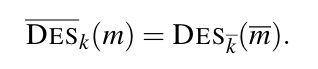
\includegraphics[width=0.25\linewidth]{formula1}
\caption{\label{fig:form1} Formula for DES complementation property}
\end{figure}

Weak keys are four special keys follow the property that DES encrypts a message twice with the same weak keys will return
the same message shown in Figure~\ref{fig:form2}. It is because the weak keys cause round keys equal to  the reverse of
the round keys, cause the DES encryption and decryption to be the same. Weak keys also have the property that each weak key
has corresponding $2^{32}$ messages that encrypt these messages with that weak key will result message unchanged. These messages
have the property that their input halves are the same in the encryption process of the 8th rounds. By combining this with the weak keys' reverse
order round keys property, it ensures the input halves in the (8-n)th and (8+n)th round are the same, result the original message (0th round) the same
as the ciphertext (16th round).

\begin{figure}
\centering
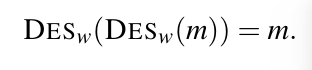
\includegraphics[width=0.25\linewidth]{formula2}
\caption{\label{fig:form2} Formula for Weak key property}
\end{figure}

Similarly, semi-weak keys are six key pairs that encrypts a message with one of the key in the pair then encrypts the resulting
ciphertext with the other key in the pair will keep the message unchanged. The formula is shown in Figure~\ref{fig:form3}. The reason
is the same as weak keys, the round keys of the two semi-weak keys in a pair are arranged in the reverse order.

\begin{figure}
\centering
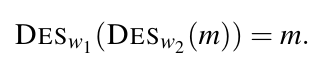
\includegraphics[width=0.25\linewidth]{formula3}
\caption{\label{fig:form3} Formula for Semi-weak key property}
\end{figure}

These properties cannot reduce the complexity for exhaustive key search especially for only 4 weak keys compare to the total
of $2^{56}$ keys. However, their existence can be vital when DES is used within some construction[3].

\subsection{DES in HOL4}
DES algorithm has been built in the "desScript" file in HOL4, and my paper build the verifications based on the DES implemented
in this file.

In the file, it first defines some specific types used in
the Data Encryption Standard implementation. It includes the halves of word/plaintext as a pair of word32, halves of
keys in each round as pair of word28 and a function type of S-Box that take word6 as inputs and return
word4. It also includes the data tables to help facilitate the IP, inverse IP permutations, E expansion, P, PC1 and PC2
permutations, round-dependent rotation values and the permutation values for the S-boxes. Then there are
some functions and definitions that perform the expansion, permutations, reversion and the S-Boxes' processing. The "Key Scheduling" section
in this file are definitions to build the round keys from the input key. As the last part of preparing, there are
join and split functions to initially split the plaintext and form the result ciphertext. Theorems are also constructed to
verify some basic properties and help ensure the correctness of implementations.

It then actually build the XOR operation, round function and swap operation in each round. Moreover, it combines the above operations, along with the
round keys to form the actual process for each round and ultimately construct the complete DES process over a total of16 rounds.
It also implements a help function that can return the input halves in each round as a pair in the form of (M a, M b). It is beneficial
for any future analysis of DES, including the verification of the proper DES implementation in "desScript" and my additional DES
properties proving. At last, it proved that as a Feistel network, the implemented encryption of DES using the round
keys, followed by a second encryption using the reversed round keys will return the original plaintext.

Consequently, it not only verifies that the decryption of DES is the same process of encryption but with reversed round keys,
but also confirms the correctness of DES implementation in HOL4 by proving that decrypting the encrypted message with the same key
will return the original message.

\section{DES property in HOL4}
In my $des_propScript$ file in HOL4, there are some basic settings. It loads all the relevant theories and libraries which contains
necessary definitions and theorems I need to use including the $desScript$. I set the $guessing\_word\_lengths$ to true so that
I do not need to set the length for each word, they will be assigned to a length based on the conditions. Additionally, I also define a simpleset
$fcp\_ss$, it is a simplification set that combines $std\_ss$, the basic simplification set, with $FCP\_ss$, the simpset fragment
specifically simplifies finite Cartesian product expressions.

\subsection{Complementation property}
First of all, I proved the complementation property, it is implemented as the theorem $comple\_property$.

\begin{alltt}
\HOLTokenTurnstile{} \HOLNumLit{0} \HOLSymConst{\HOLTokenLt{}} \HOLFreeVar{n} \HOLSymConst{\HOLTokenConj{}} \HOLFreeVar{n} \HOLSymConst{\HOLTokenLt{}} \HOLNumLit{17} \HOLSymConst{\HOLTokenConj{}} \HOLConst{DES} \HOLFreeVar{n} \HOLFreeVar{k} \HOLSymConst{=} (\HOLFreeVar{encrypt}\HOLSymConst{,}\HOLFreeVar{decrypt}) \HOLSymConst{\HOLTokenConj{}}
   \HOLConst{DES} \HOLFreeVar{n} (\HOLSymConst{\HOLTokenNeg{}}\HOLFreeVar{k}) \HOLSymConst{=} (\ensuremath{\HOLFreeVar{encrypt}\sp{\prime{}}}\HOLSymConst{,}\ensuremath{\HOLFreeVar{decrypt}\sp{\prime{}}}) \HOLSymConst{\HOLTokenImp{}}
   \HOLSymConst{\HOLTokenNeg{}}\HOLFreeVar{encrypt} \HOLFreeVar{m} \HOLSymConst{=} \ensuremath{\HOLFreeVar{encrypt}\sp{\prime{}}} (\HOLSymConst{\HOLTokenNeg{}}\HOLFreeVar{m})
\end{alltt}

It means for any key k, message m and number of rounds n, the complementation of encryption using m and k is the
same as the encryption using the complementation of m and k.

I initially convert the $encrypt$ function to more detailed components functions including inverse of initial permutation,
join, swap, round, split and initial permutation functions. This allows the use of rewriting rules on separated
functions. This includes some theorems proving the complementation property of each individual function mentioned above.
The below theorem is an example for join function.

\begin{alltt}
   \HOLTokenTurnstile{} \HOLConst{Join} (\HOLSymConst{\HOLTokenNeg{}}\HOLFreeVar{m}\HOLSymConst{,}\HOLSymConst{\HOLTokenNeg{}}\HOLFreeVar{n}) \HOLSymConst{=} \HOLSymConst{\HOLTokenNeg{}}\HOLConst{Join} (\HOLFreeVar{m}\HOLSymConst{,}\HOLFreeVar{n})
\end{alltt}

I then convert the $Round$ function to the $(M \,a,\; M \,b)$ by the $half\_message$ help function, so that I can research on each 32-bit
half of the block and use the relation between halves in the same and different rounds. Moreover, I simplify the proving goals by rewriting it with the theorems about the complementation
property of each individual function, leave only solving the complementation property of a pair of M function.
\begin{multline}
(M \; (u', v') \; keys' \; n, \; M \; (u', v') \; keys' \; (SUC \, n)) \\
= (\sim M \; (u, v) \; keys \; n, \; \sim M \; (u, v) \; keys \; (SUC \, n))
\end{multline}

I decide to use the Mathematical induction method using $Induct\_on$ in HOL4. I replace the variable n to x, define x to be $<=$ n, and then
perform induction on variable x. It is to avoid the failure of proving the induction step. As the prerequisite of using
given case is $n>0$ , but in the step case, only $(SUC n) > 0$ (SUC means successor) is given. From $n+1 > 0$, it is not possible to
derive the requirement of $n > 0$, thus given case cannot be used, verification cannot be pushed further. By converting to x,
the prerequisites can be easily meet, and facilitating the proof process.

To prove the base case, we only need to convert back to the form of $Round$ function and use the base case of the $Round$ function.
It is because only $Round$ function is built using the relationships between its values based on inductively given inputs, and
it has the base case for $x=0$. To complete the
base case verification, I also prove $(u,\;v)= (u',\;v')$ by extract the abbreviation of them back into their original forms, and apply the complementation rule of
IP function. The abbreviation can be viewed below~\ref{fig:form4}.

\begin{figure}
\centering
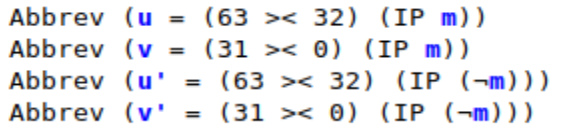
\includegraphics[width=0.25\linewidth]{abbr1}
\caption{\label{fig:form4} The abbreviation}
\end{figure}

It is important to note that $(M \,a,\;M \,b)$ can be converted from the $Round$ function. It is defined as a pair of two
halves taking $n$th round as one of the inputs,
which are the two halves in the n-th round during the DES encryption process. According to the workflow of encryption, the right
half of round $n$ equals to the left half of round $n+1$ by the swap operation at the end of each round. Depend on this and the workflow,
the right half of round $n+1$ can be expressed as the two halves in previous round with some operations.
By using the relationship of halves between different rounds,
each half of $(M \,a,\;M \,b)$ in round $n+1$ can be expressed by the halves in round $n$. Consequently, in the induction step,
the step case which contains $(M \,a,\;M \,b)$ in round $SUC \,n$ can be expressed into formulas using $(M \,a,\;M \,b)$ in round
$n$ which are contained in the base case. As a result, I can use the assumptions provided in the base case to push forward my
verification.

\begin{multline}
Assumption: \quad (M \; (u', v') \; keys' \; x, \; M \; (u', v') \; keys' \; (SUC \, x)) \\
= (\sim M \; (u, v) \; keys \; x, \; \sim M \; (u, v) \; keys \; (SUC \, x))
\end{multline}

\begin{multline}
Goal: \quad (M \; (u', v') \; keys' \; (SUC \,x), \; M \; (u', v') \; keys' \; (SUC \,(SUC \, x))) \\
= (\sim M \; (u, v) \; keys \; (SUC \,x), \; \sim M \; (u, v) \; keys \; (SUC \,(SUC \, x)))
\end{multline}

By the above conversions and simplifications using base case, the proving goal is now transformed to verify only the
complementation property about round function. It is to prove that round function with 32-bite message m and round
key generated by key k equals to the round function with inputs of
the complementation of both m and k. In HOL4, $RoundOp$ function is built to represent round function of each round
combining the expansion E, XOR operation with round key, S-boxes permutations S and the bit-level permutation P. By expanding
the $RoundOp$ function, the goal can now reduce to:

\begin{multline}
P \; (S \; (E \;(\sim M \; (u, v) \; keys \; (x+1)) \; \oplus \; (EL \;x \;keys')))\\
= P \; (S \; (E \;(M \; (u, v) \; keys \; (x+1)) \;\oplus \;(EL \;x \;keys)))
\end{multline}

As the property of exclusive OR operation, $\sim \; a \; \oplus \; \sim \; b \;= \;a \; \oplus \; b$ and the support
complementation property of the expansion function, $E \; (\sim \; a) \;= \; \sim \; E \; (a)$ once I prove the complementation of
round key generated by key k is equal to the round key generated by the complementation of key k, the verification of complementation property
in DES is done.

The implementation of the design about round key in HOL4 is generated by $RoundKey$ and $KS$ function. $RoundKey$ outputs a
round key list that the elements in it
are pairs of 28-bit words, each pair represents the two halves after the splitting of initial key, the rearrangement by PC1
and the rotation in different rounds. $KS$ then using the $MAP$ function to map each element in the output of $RoundKey$ to
perform PC2 permutations. For convenience in the verification, I define three functions $RK$, $RK\_L$ and $RK\_R$.
$RoundKey$ can be converted to $RK$ and thus split into $(RK\_L \; a \;,RK\_R \; a)$, and now I can work on each half of the pair
separately, instead of only be able to work on the pair as a whole. The current form of goal can be expressed like:

\begin{multline}
EL \; x \; (MAP \; f \; (list \; of \; input \; \sim k))\\
= \sim EL \; x \; (MAP \; f \; (list \; of \; input \; k))
\end{multline}

By applying a series of rewriting rules in $listTheory$ that can deal with $EL$, $MAP$ and some functions in $f$, the complementation
theorems for $RK\_L$ and $RK\_R$, the goal finally transforms to $MAP\; f \;l = MAP\; f'\; l$. At last, the complementation property of PC2
permutation is used
to finish the proof of $f\;=\;f'$. The initial goal of DES complementation property is proved in HOL4 through the above steps.

As mentioned above, I proved many support theorems about the complementation property of each single operation, their proofs are
done in a similar way. The operations are expanded by their definitions to transform the verification into each bit of $\sim m$
at the permuted indices equals to the complementation of each bit of $m$ in the same indices. For example, the indices of IP
permutation are transformed to $64 \; - \; EL \; (63 \;-\;i) \; IP_{data}$ where $i$ is the original index of m before IP
permutation. $IP_{data}$ is the IP table to do the permutations, and it rearranges the bits in different positions of m
to form a new message. Then I need to prove that the transformed indices are still less than the length of input message m to
meet the prerequisite for using the theorem, $FCP\_BETA$ and then I can complete the proof.

\begin{alltt}
   \HOLTokenTurnstile{} \HOLFreeVar{i} \HOLSymConst{\HOLTokenLt{}} \HOLConst{dimindex} (:\ensuremath{\beta}) \HOLSymConst{\HOLTokenImp{}} (\HOLSymConst{FCP}) \HOLFreeVar{g} \HOLConst{'} \HOLFreeVar{i} \HOLSymConst{=} \HOLFreeVar{g} \HOLFreeVar{i}
\end{alltt}

The proof that the transformed indices are all less than the length of input message m (64) given $i$ is less than 64 uses
the method of exhaustion. It repeatedly proves the transformed index is less than 64 for each value of i for 64 times, covering
all cases from i=0 to i=63. The proof is completed as all 64 situations meet the condition. Overall, the support theorems are
all proved with a similar way.

There are some special built-in tactics, conversions used here. The \\
$MATCH\_MP\_TAC$ tactic takes a theorem as input,
it can be applied to the goal if the current goal is in the form of the consequent of this theorem. The goal can then be
converted to the antecedent of the theorem. $rpt$ is a tactic that takes a tactic as input and repeatedly apply the tactic until
it no longer succeeds. $CONV\_TAC$ is a special tactic that makes a tactic from a conversion. Then $BOUNDED\_FORALL\_CONV$ is a
conversion that deal with universal quantification for bounded natural numbers, so it converts $\forall n. \;n \; < \; k$ to
the conjunction of $n=0$ to $n=k-1$, like the exhaustion methods for i that I mentioned above.

There are also some theorems and definitions that are frequently used in the proof. $word_1comp_def$ defines the complementation of a word m
$\sim m$ equals to the concentration of the complementation of each bit of word m. It helps deal with the complementation in
bit level.

\begin{alltt}
   \HOLTokenTurnstile{} \HOLSymConst{\HOLTokenNeg{}}\HOLFreeVar{w} \HOLSymConst{=} \HOLConst{FCP} \HOLBoundVar{i}. \HOLSymConst{\HOLTokenNeg{}}\HOLFreeVar{w} \HOLConst{'} \HOLBoundVar{i}
\end{alltt}

When dealing with the lists and some operations applies to lists like the map function. $MAP\_TL$ shows that applying a function
to the tail of a list is equal to the tail of a list after the mapping. Then the theorem $MAP\_MAP\_o$ states applying two functions
to a list using $MAP$ twice is equivalent to applying the composition of the two function using $MAP$ once.


\begin{alltt}
   \HOLTokenTurnstile{} \HOLConst{MAP} \HOLFreeVar{f} (\HOLConst{TL} \HOLFreeVar{l}) \HOLSymConst{=} \HOLConst{TL} (\HOLConst{MAP} \HOLFreeVar{f} \HOLFreeVar{l})
\end{alltt}

\begin{alltt}
   \HOLTokenTurnstile{} \HOLConst{MAP} \HOLFreeVar{f} (\HOLConst{MAP} \HOLFreeVar{g} \HOLFreeVar{l}) \HOLSymConst{=} \HOLConst{MAP} (\HOLFreeVar{f} \HOLSymConst{\HOLTokenCompose} \HOLFreeVar{g}) \HOLFreeVar{l}
\end{alltt}

\subsection{Weak and semi-weak key property}
I first define the four weak keys into HOL4 in hexadecimal form. Then I want to prove in HOL4 that for all the DES encryptions using
the weak keys, applying the encryption twice to any message will result the message nochange.

\begin{alltt}
   \HOLTokenTurnstile{} \HOLConst{MEM} \HOLFreeVar{k} \HOLConst{Wkey} \HOLSymConst{\HOLTokenConj{}} \HOLConst{FullDES} \HOLFreeVar{k} \HOLSymConst{=} (\HOLFreeVar{encrypt}\HOLSymConst{,}\HOLFreeVar{decrypt}) \HOLSymConst{\HOLTokenImp{}}
   \HOLFreeVar{encrypt} (\HOLFreeVar{encrypt} \HOLFreeVar{plaintext}) \HOLSymConst{=} \HOLFreeVar{plaintext}
\end{alltt}

It can be proven easily using the existing theorem $desCore\_CORRECT$ in $desTheory$. DES has the property that
the decryption in DES of a key is the same process of encryption in DES but use the reverse list of round keys generated
from the same key. The $desCore\_CORRECT$ theorem uses this property and the fact that decrypting an encrypted message
returns the original message. It successfully proves that encryption to a message twice with a key,
once using the normal round keys, once using the round keys in reverse order remains message unchanged.

\begin{alltt}
   \HOLTokenTurnstile{} \HOLConst{LENGTH} \HOLFreeVar{keys} \HOLSymConst{=} \HOLFreeVar{r} \HOLSymConst{\HOLTokenImp{}}
   \HOLConst{desCore} \HOLFreeVar{r} (\HOLConst{REVERSE} \HOLFreeVar{keys}) (\HOLConst{desCore} \HOLFreeVar{r} \HOLFreeVar{keys} \HOLFreeVar{plaintext}) \HOLSymConst{=}
   \HOLFreeVar{plaintext}
\end{alltt}

By applying this to the goal, I am left with only the proofing of the prerequisite of $desCore\_CORRECT$ and the
proof of round keys list generated by weak key remains the same after being reversed, that is:

\begin{equation}
\begin{split}
   REVERSE \; (KS \; k \; 16) &= KS \; k \; 16
\end{split}
\end{equation}


The rest part is easy to prove, the length of the list of round keys is equal to the number of rounds by the $LENGTH\_KS$
theorem. The equivalent proof about the round keys can be done by substituting each weak key's value into the goal,
use the $EVAL\_TAC$ that applies the values of keys to the goal and evaluate on the value. The goal is proved after
the successful equation calculation on each value.

\begin{alltt}
   \HOLTokenTurnstile{} \HOLConst{LENGTH} (\HOLConst{KS} \HOLFreeVar{k} \HOLFreeVar{n}) \HOLSymConst{=} \HOLFreeVar{n}
\end{alltt}

The semi-weak keys' property and its corresponding verification are similar to weak keys'. I define them as pairs in a list,
set the goal to be: encrypting a message with one key in a pair and encrypting the ciphertext with another key
in that pair make the ciphertext back to the original message.

\begin{alltt}
   \HOLTokenTurnstile{} \HOLConst{MEM} \HOLFreeVar{pair} \HOLConst{Semiwkey} \HOLSymConst{\HOLTokenConj{}} \HOLFreeVar{pair} \HOLSymConst{=} (\ensuremath{\HOLFreeVar{s}\sb{\mathrm{1}}}\HOLSymConst{,}\ensuremath{\HOLFreeVar{s}\sb{\mathrm{2}}}) \HOLSymConst{\HOLTokenConj{}}
   \HOLConst{FullDES} \ensuremath{\HOLFreeVar{s}\sb{\mathrm{1}}} \HOLSymConst{=} (\HOLFreeVar{encrypt}\HOLSymConst{,}\HOLFreeVar{decrypt}) \HOLSymConst{\HOLTokenConj{}}
   \HOLConst{FullDES} \ensuremath{\HOLFreeVar{s}\sb{\mathrm{2}}} \HOLSymConst{=} (\ensuremath{\HOLFreeVar{encrypt}\sp{\prime{}}}\HOLSymConst{,}\ensuremath{\HOLFreeVar{decrypt}\sp{\prime{}}}) \HOLSymConst{\HOLTokenImp{}}
   \HOLFreeVar{encrypt} (\ensuremath{\HOLFreeVar{encrypt}\sp{\prime{}}} \HOLFreeVar{plaintext}) \HOLSymConst{=} \HOLFreeVar{plaintext}
\end{alltt}

\begin{alltt}
   \HOLTokenTurnstile{} \HOLConst{MEM} \HOLFreeVar{pair} \HOLConst{Semiwkey} \HOLSymConst{\HOLTokenConj{}} \HOLFreeVar{pair} \HOLSymConst{=} (\ensuremath{\HOLFreeVar{s}\sb{\mathrm{1}}}\HOLSymConst{,}\ensuremath{\HOLFreeVar{s}\sb{\mathrm{2}}}) \HOLSymConst{\HOLTokenConj{}}
   \HOLConst{FullDES} \ensuremath{\HOLFreeVar{s}\sb{\mathrm{1}}} \HOLSymConst{=} (\HOLFreeVar{encrypt}\HOLSymConst{,}\HOLFreeVar{decrypt}) \HOLSymConst{\HOLTokenConj{}}
   \HOLConst{FullDES} \ensuremath{\HOLFreeVar{s}\sb{\mathrm{2}}} \HOLSymConst{=} (\ensuremath{\HOLFreeVar{encrypt}\sp{\prime{}}}\HOLSymConst{,}\ensuremath{\HOLFreeVar{decrypt}\sp{\prime{}}}) \HOLSymConst{\HOLTokenImp{}}
   \ensuremath{\HOLFreeVar{encrypt}\sp{\prime{}}} (\HOLFreeVar{encrypt} \HOLFreeVar{plaintext}) \HOLSymConst{=} \HOLFreeVar{plaintext}
\end{alltt}

The way to achieve this goal only change the part about the equivalent proof of round keys and reversed round keys.
It is now to verify that the round keys generated by one of the semi-weak keys are equal to the revered round
keys generated by the other key. The method of verification is still use $EVAL\_TAC$ to evaluate on the values of semi-weak
keys. The proof is then done.

\begin{equation}
\begin{split}
 REVERSE \; (KS \; k1 \; 16)= KS \; k2 \; 16
\end{split}
\end{equation}

\subsection{Fixed points for DES weak keys}
I can now prove each weak key has $2^{32}$ messages that encrypting these messages with the corresponding weak key remain
the messages unchanged. As mentioned in earlier section, these messages have this property based on their property that
the input halves are the same in round 8 during the DES encryption using the corresponding weak key. Based on this, I define
four sets for four weak keys that each list obtains messages with the above property. I can then prove separately that
all messages in the set meet the property that encryption does not change the message, and each set has cardinality
of $2^{32}$.

\begin{alltt}
   \HOLTokenTurnstile{} \HOLFreeVar{x} \HOLSymConst{\HOLTokenIn{}} \HOLConst{Wtext1} \HOLSymConst{\HOLTokenConj{}} \HOLConst{FullDES} \HOLConst{Wkey1} \HOLSymConst{=} (\HOLFreeVar{encrypt}\HOLSymConst{,}\HOLFreeVar{decrypt}) \HOLSymConst{\HOLTokenImp{}}
   \HOLFreeVar{encrypt} \HOLFreeVar{x} \HOLSymConst{=} \HOLFreeVar{x}
\end{alltt}

\begin{alltt}
   \HOLTokenTurnstile{} \HOLFreeVar{x} \HOLSymConst{\HOLTokenIn{}} \HOLConst{Wtext2} \HOLSymConst{\HOLTokenConj{}} \HOLConst{FullDES} \HOLConst{Wkey2} \HOLSymConst{=} (\HOLFreeVar{encrypt}\HOLSymConst{,}\HOLFreeVar{decrypt}) \HOLSymConst{\HOLTokenImp{}}
   \HOLFreeVar{encrypt} \HOLFreeVar{x} \HOLSymConst{=} \HOLFreeVar{x}
\end{alltt}

\begin{alltt}
   \HOLTokenTurnstile{} \HOLFreeVar{x} \HOLSymConst{\HOLTokenIn{}} \HOLConst{Wtext3} \HOLSymConst{\HOLTokenConj{}} \HOLConst{FullDES} \HOLConst{Wkey3} \HOLSymConst{=} (\HOLFreeVar{encrypt}\HOLSymConst{,}\HOLFreeVar{decrypt}) \HOLSymConst{\HOLTokenImp{}}
   \HOLFreeVar{encrypt} \HOLFreeVar{x} \HOLSymConst{=} \HOLFreeVar{x}
\end{alltt}

\begin{alltt}
   \HOLTokenTurnstile{} \HOLFreeVar{x} \HOLSymConst{\HOLTokenIn{}} \HOLConst{Wtext4} \HOLSymConst{\HOLTokenConj{}} \HOLConst{FullDES} \HOLConst{Wkey4} \HOLSymConst{=} (\HOLFreeVar{encrypt}\HOLSymConst{,}\HOLFreeVar{decrypt}) \HOLSymConst{\HOLTokenImp{}}
   \HOLFreeVar{encrypt} \HOLFreeVar{x} \HOLSymConst{=} \HOLFreeVar{x}
\end{alltt}

First, to prove DES encryption with messages in the set remains message unchanged, I expand the goal to more detailed operations
during the DES encryption process. I find that only
if I proved that the reverse of the halves in round 16 during the encryption process are equal to the halves in round 0,
the rest of the proof is
quite simple. I can use the halves in round 0 which do not process any round function, but only the inital IP permutation
and splitting to simplify the goal to:

\begin{equation}
\begin{split}
 IIP \; (Join \; (Split \; (IP \; x))) \; = \; x
\end{split}
\end{equation}

These operations can be easily cancelled out by each other using theorem $IIP\_IP\_Inverse$ nad $Join\_Split\_Inverse$.

\begin{alltt}
   \HOLTokenTurnstile{} \HOLConst{IIP} (\HOLConst{IP} \HOLFreeVar{w}) \HOLSymConst{=} \HOLFreeVar{w}
\end{alltt}

\begin{alltt}
   \HOLTokenTurnstile{} \HOLConst{Join} (\HOLConst{Split} \HOLFreeVar{w}) \HOLSymConst{=} \HOLFreeVar{w}
\end{alltt}

I am now left to prove the support theorem $weakK\_sup$ given the property of each set. It is hard to compare two pairs of
halves that differ by sixteen rounds of operations directly. To achieve the goal in HOL4, I build the support theorem
$weakK\_sup$ by setting the goal to show that for be each pair of halves in (8-n) round is equal to the reversed pair
in round (8+n). I can then use proof by induction on $n$ to complete the proof.

\begin{alltt}
   \HOLTokenTurnstile{} \HOLConst{MEM} \HOLFreeVar{k} \HOLConst{Wkey} \HOLSymConst{\HOLTokenConj{}} \HOLNumLit{0} \HOLSymConst{\HOLTokenLeq{}} \HOLFreeVar{n} \HOLSymConst{\HOLTokenConj{}} \HOLFreeVar{n} \HOLSymConst{\HOLTokenLeq{}} \HOLNumLit{8} \HOLSymConst{\HOLTokenConj{}}
   \HOLConst{Split} (\HOLConst{IP} (\HOLConst{desCore} \HOLNumLit{8} (\HOLConst{KS} \HOLFreeVar{k} \HOLNumLit{8}) \HOLFreeVar{x})) \HOLSymConst{=} (\HOLFreeVar{w}\HOLSymConst{,}\HOLFreeVar{w}) \HOLSymConst{\HOLTokenImp{}}
   \HOLConst{Round} (\HOLNumLit{8} \HOLSymConst{\ensuremath{-}} \HOLFreeVar{n}) (\HOLConst{KS} \HOLFreeVar{k} \HOLNumLit{16}) (\HOLConst{Split} (\HOLConst{IP} \HOLFreeVar{x})) \HOLSymConst{=}
   \HOLConst{Swap} (\HOLConst{Round} (\HOLNumLit{8} \HOLSymConst{\ensuremath{+}} \HOLFreeVar{n}) (\HOLConst{KS} \HOLFreeVar{k} \HOLNumLit{16}) (\HOLConst{Split} (\HOLConst{IP} \HOLFreeVar{x})))
\end{alltt}

As I define the message sets using round keys list contains only up to the $8th$ round to facilitate future verification,
I first prove that doing the encryption with only 8 round keys is the same as encrypt with all 16 round keys
when just encrypting for 8 rounds by another support theorem. By using it, I convert the prerequisite to mathch the
round keys list with the goal.

Then I start the induction on n and the base case is to prove the two equal input halves $(w\;,\;w)$ at round n is the same after
swapping. It is straightforward, and I only need to expand the $Round$ function to pair form and apply the $Swap$ definition.

For the induction step, I know the base case shows that the reversed halves in round $a$ $(Ra\;,\; La)$ are equal to
the halves in round $b$ $(Lb\;,\;Rb)$ where $a$ and $b$ represents $8+n$ and $8-n$.
To proving the step case, I can directly get the right half of round $(b-1)$ $R(b-1)$ is equal to the left half of round $b$
$Lb$ and
the left half of round $(a+1)$ $L(a+1)$ is equal to the right half of round $a$ $Ra$ because only swap operation happens on
these halves between rounds. As $Ra\;= \; Lb$ by the base case, I can get $R(b-1)$ and $L(a+1)$ are the same.
Then because the encryption and decryption process of DES are the same, I can get $L(b-1)$ back from halves in round $b$ through
the round function $f(b-1)$ by using the swap operation, round function and XOR operation

\begin{equation}
\begin{split}
   L(b-1) \; = \; (Rb \; \oplus \; f(b-1)\,(\;Lb\;)
\end{split}
\end{equation}
$R(a+1)$ can also be represented by $Ra$ and $La$ in normal encryption manner through the round function $f(a+1)$

\begin{equation}
\begin{split}
   R(a+1) \; = \; La \; \oplus \; f(a+1)\,(\;Ra\;)
\end{split}
\end{equation}
According to the proof
done above that round keys list generated by a weak key remains the same after being reversed, I can conclude that the list
is  symmetric, and thus the $(b-1)$th and $(a+1)$th round keys are the same in the round keys list of length 16.
The round function $f(b-1)$ and $f(a+1)$ are then the same as round key is the only change variable for round functions in different
rounds. By combining this with $Rb\;= \; La$ and $Lb\;= \; Ra$, $L(b-1)$ and $R(a+1)$ are the same, and we can prove the step
case is also right given the base case.

Using the above way in HOL4, I convert the goal to halves using $(M\;a\;,\;M\;b)$ function and then
express the step case' halves using the base cases' halves. The only goal left is the proof of the elements in
symmetric positions are the same. I need to put each weak key's value into the goal, calculate the generated
round keys list for each key, ensure the step case's index do not exceed the length of list. At last, I need to
do the method of exhaustion, examine each possible value of n from 0 to 15 to check if they meet the goal because of
the lack of theorems in HOL4 on this aspect. The support theorem is proved.

\begin{equation}
\begin{split}
 EL \; (7-n) \; (KS \; k \; 16) = EL \; (n+8) \; (KS \; k \; 16)
\end{split}
\end{equation}
Switch to the last support theorem $wkey1\_equal$ mentioned above. It is also proved by induction, the base case can
be directly proved by the base case of $Round$. The indcution step is proved in the same way as above by transforming
the $Round$ function to $(M\;a\;,\;M\;b)$ form first and then express the step case' halves using the base cases' halves.
The last part of verification is also examine each possible value of n to the goal, use the method of exhaustion to
test all situations meet the goal and the theorem is proved.

\begin{alltt}
   \HOLTokenTurnstile{} \HOLConst{MEM} \HOLFreeVar{k} \HOLConst{Wkey} \HOLSymConst{\HOLTokenConj{}} \HOLFreeVar{n} \HOLSymConst{\HOLTokenLeq{}} \HOLNumLit{8} \HOLSymConst{\HOLTokenImp{}}
   \HOLConst{Round} \HOLFreeVar{n} (\HOLConst{KS} \HOLFreeVar{k} \HOLNumLit{8}) (\HOLConst{Split} \HOLFreeVar{x}) \HOLSymConst{=} \HOLConst{Round} \HOLFreeVar{n} (\HOLConst{KS} \HOLFreeVar{k} \HOLNumLit{16}) (\HOLConst{Split} \HOLFreeVar{x})
\end{alltt}

It is time to prove that the cardinality of the sets of these messages is $2^{32}$. I show these sets form bijection with
the universal set of 32-bit words first. To achieve these, I define two functions for each set, one of the two can map the messages
set to the universal set and the other can map reversely.

\begin{alltt}
   \HOLTokenTurnstile{} \HOLConst{BIJ} \HOLConst{w1trans1} \HOLConst{Wtext1} \ensuremath{{\cal{U}}}(:\HOLTyOp{word32})
\end{alltt}

\begin{alltt}
   \HOLTokenTurnstile{} \HOLConst{BIJ} \HOLConst{w2trans1} \HOLConst{Wtext2} \ensuremath{{\cal{U}}}(:\HOLTyOp{word32})
\end{alltt}

\begin{alltt}
   \HOLTokenTurnstile{} \HOLConst{BIJ} \HOLConst{w3trans1} \HOLConst{Wtext3} \ensuremath{{\cal{U}}}(:\HOLTyOp{word32})
\end{alltt}

\begin{alltt}
   \HOLTokenTurnstile{} \HOLConst{BIJ} \HOLConst{w4trans1} \HOLConst{Wtext4} \ensuremath{{\cal{U}}}(:\HOLTyOp{word32})
\end{alltt}

To prove the bijection relation between the two sets, $BIJ\_IFF\_INV$ theorem can be used to convert the $BIJ$ function into
four sub-goals. It includes proving that all elements in messages set belongs to the other universal set of word32 after mapping,
and vice versa. Moreover, the other two goals are applying the two functions together to the sets will keep the elements unchanged.

\begin{alltt}
   \HOLTokenTurnstile{} \HOLConst{BIJ} \HOLFreeVar{f} \HOLFreeVar{s} \HOLFreeVar{t} \HOLSymConst{\HOLTokenEquiv{}}
   (\HOLSymConst{\HOLTokenForall{}}\HOLBoundVar{x}. \HOLBoundVar{x} \HOLSymConst{\HOLTokenIn{}} \HOLFreeVar{s} \HOLSymConst{\HOLTokenImp{}} \HOLFreeVar{f} \HOLBoundVar{x} \HOLSymConst{\HOLTokenIn{}} \HOLFreeVar{t}) \HOLSymConst{\HOLTokenConj{}}
   \HOLSymConst{\HOLTokenExists{}}\HOLBoundVar{g}. (\HOLSymConst{\HOLTokenForall{}}\HOLBoundVar{x}. \HOLBoundVar{x} \HOLSymConst{\HOLTokenIn{}} \HOLFreeVar{t} \HOLSymConst{\HOLTokenImp{}} \HOLBoundVar{g} \HOLBoundVar{x} \HOLSymConst{\HOLTokenIn{}} \HOLFreeVar{s}) \HOLSymConst{\HOLTokenConj{}} (\HOLSymConst{\HOLTokenForall{}}\HOLBoundVar{x}. \HOLBoundVar{x} \HOLSymConst{\HOLTokenIn{}} \HOLFreeVar{s} \HOLSymConst{\HOLTokenImp{}} \HOLBoundVar{g} (\HOLFreeVar{f} \HOLBoundVar{x}) \HOLSymConst{=} \HOLBoundVar{x}) \HOLSymConst{\HOLTokenConj{}}
       \HOLSymConst{\HOLTokenForall{}}\HOLBoundVar{x}. \HOLBoundVar{x} \HOLSymConst{\HOLTokenIn{}} \HOLFreeVar{t} \HOLSymConst{\HOLTokenImp{}} \HOLFreeVar{f} (\HOLBoundVar{g} \HOLBoundVar{x}) \HOLSymConst{=} \HOLBoundVar{x}
\end{alltt}

Taking the example for proving the first weak key, and the other weak keys are all proved in the same way. Their corresponding
sets and functions just change the weak key used.
The first sub-goal that all elements in messages set belongs to the other universal set of word32 after function $w1trans1$ is
proved directly. It takes the 64-bit messages as inputs and outputs only the first reversed halves of message encrypted by 8
rounds. As the outputs are 32 bits, they surely belong to the universal set of word32.

\begin{alltt}
   \HOLTokenTurnstile{} \HOLConst{w1trans1} \HOLFreeVar{x} \HOLSymConst{=} \HOLConst{FST} (\HOLConst{Split} (\HOLConst{IP} (\HOLConst{desCore} \HOLNumLit{8} (\HOLConst{KS} \HOLConst{Wkey1} \HOLNumLit{8}) \HOLFreeVar{x})))
\end{alltt}

The second sub-goal can be converted using definition of function $w1trans2$ and set $Wtext1$. All 32-bit messages
(in universal set of word32) are formed as a pair of equal halves, applied with $Join$ and $IIP$ operation, encrypted
for 8 rounds twice, and applied with $IP$ and $Split$ operation. And to prove the result halves are still the same.

\begin{alltt}
   \HOLTokenTurnstile{} \HOLConst{w1trans2} \HOLFreeVar{x} \HOLSymConst{=} \HOLConst{desCore} \HOLNumLit{8} (\HOLConst{KS} \HOLConst{Wkey1} \HOLNumLit{8}) (\HOLConst{IIP} (\HOLConst{Join} (\HOLFreeVar{x}\HOLSymConst{,}\HOLFreeVar{x})))
\end{alltt}

\begin{alltt}
   \HOLTokenTurnstile{} \HOLConst{Wtext1} \HOLSymConst{=}
   \HOLTokenLeftbrace{}\HOLBoundVar{x} \HOLTokenBar{} \HOLSymConst{\HOLTokenExists{}}\HOLBoundVar{w}. \HOLConst{Split} (\HOLConst{IP} (\HOLConst{desCore} \HOLNumLit{8} (\HOLConst{KS} \HOLConst{Wkey1} \HOLNumLit{8}) \HOLBoundVar{x})) \HOLSymConst{=} (\HOLBoundVar{w}\HOLSymConst{,}\HOLBoundVar{w})\HOLTokenRightbrace{}
\end{alltt}

I can also use the previous method to help the proof, the two encryptions of 8 rounds with the weak key cancel each other out
as one of the encryption can be treated as decryption. The $Split$ and $Join$ operations can be cancelled out, and also the
$IP$ and $IIP$ operations, results the initial pair of haves unchanged, so the two halves must remain the same with no change.
The second sub-goal is then proved.

The third sub-goal is to prove for an element in the messages' set with the described property, when they are converted
tp the 32-bit half through $w1trans1$, formed as a pair of equal halves and map with the $w1trans2$, the result messages
remain the same~\ref{fig:form5}. It proves with the same way as sub-goal 2, but begins to cancell out the $Join$ and $Split$ operation first, then
the $IIP$ and $IP$ operations and at last the two encryption processes with weak key. It also cancells each other out,
but in a different order.

\begin{figure}
\centering
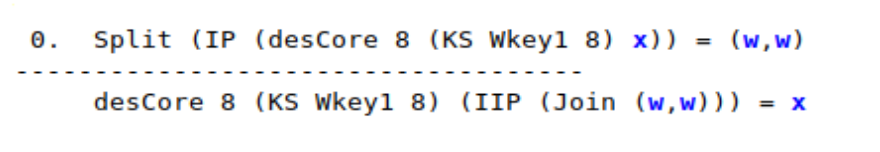
\includegraphics[width=0.25\linewidth]{BIJ}
\caption{\label{fig:form5} Apply two functions to elements in Wtext1}
\end{figure}

The elements are initially in the universal set, change to pairs equal halves, and apply the $w1trans2$ function followed
by the $w1trans1$ function in the last sub-goal. It can also be verified by cancelling each operations in another order.
The bijection relation between two sets is finally proved.

The bijection proofs for the other three keys are exactly the same, so one proof $BIJ\_for\_weak\_keys\_explicit$ with the lists of sets, functions and
weak keys as inputs can be done using the existing seperate BIJ theorems.

\begin{alltt}
   \HOLTokenTurnstile{} \HOLFreeVar{i} \HOLSymConst{\HOLTokenLt{}} \HOLNumLit{4} \HOLSymConst{\HOLTokenImp{}} \HOLConst{BIJ} (\HOLConst{EL} \HOLFreeVar{i} \HOLConst{wtrans1}) (\HOLConst{EL} \HOLFreeVar{i} \HOLConst{Wtextlist}) \ensuremath{{\cal{U}}}(:\HOLTyOp{word32})
\end{alltt}

The universal set of word32 has the cardinality of $2^{32}$ by the theorem \\
$card\_word32$. As a result, by proving that
these sets have the same cardinality as the universal set of word32, I can then prove the cardinality of each message set
is $2^{32}$. I can meet the prerequisites that the universal set of word32 is finite directly and use the above
bijection relation, then theorem $FINITE\_BIJ\_CARD$ can be used to prove the equivalence of cardinality.

\begin{alltt}
   \HOLTokenTurnstile{} \HOLConst{CARD} \ensuremath{{\cal{U}}}(:\HOLTyOp{word32}) \HOLSymConst{=} \HOLNumLit{2} \HOLSymConst{\HOLTokenExp{}} \HOLNumLit{32}
\end{alltt}

\begin{alltt}
   \HOLTokenTurnstile{} \HOLConst{FINITE} \HOLFreeVar{s} \HOLSymConst{\HOLTokenConj{}} \HOLConst{BIJ} \HOLFreeVar{f} \HOLFreeVar{s} \HOLFreeVar{t} \HOLSymConst{\HOLTokenImp{}} \HOLConst{CARD} \HOLFreeVar{s} \HOLSymConst{=} \HOLConst{CARD} \HOLFreeVar{t}
\end{alltt}

As a result, each message set is proved with cardinality of $2^{32}$ and the theorem is stored as
$DES\_weak\_fp\_card$ in $des\_propTheory$.

\begin{alltt}
   \HOLTokenTurnstile{} \HOLConst{MEM} \HOLFreeVar{x} \HOLConst{Wtextlist} \HOLSymConst{\HOLTokenImp{}} \HOLConst{CARD} \HOLFreeVar{x} \HOLSymConst{=} \HOLNumLit{2} \HOLSymConst{\HOLTokenExp{}} \HOLNumLit{32}
\end{alltt}


   a
\end{document}


